\documentclass[11pt]{article}
\usepackage{amsmath, amssymb, amsthm}
\usepackage[retainorgcmds]{IEEEtrantools}

\usepackage[pdftex]{graphicx}
\usepackage{tikz}
\usetikzlibrary{intersections}

\usepackage{marginnote}
\usepackage{endnotes}

\usepackage{fancyhdr}

%Listings stuff
\usepackage{listings}
\usepackage{lstautogobble}
\usepackage{color}

\definecolor{gray}{rgb}{0.5,0.5,0.5}
\lstset{
basicstyle={\small\ttfamily},
tabsize=3,
numbers=left,
numbersep=5pt,
numberstyle=\tiny\color{gray},
stepnumber=2,
breaklines=true
}

%Properly formatted differential 'd'
\newcommand{\ud}{\, \mathrm{d}}

%Format stuff
\pagestyle{fancy}
\headheight 35pt

%Header info
\chead{\Large \textbf{Linear Algebra}}
\lhead{}
\rhead{}

\begin{document}
\section{Gaussian Elimination}
	\marginnote{Guassian elimination?}Given a linear system of equations represented by $\mathbf{A}\vec{x} = \vec{b}$, where the matrix $\mathbf{A}$ represents the coefficients of the unknowns or variables in $\vec{x}$, it is possible with a series of basic manipulations to come up with a solution.
	
	\begin{equation}
		\left(\begin{matrix}
			a & b & c & | & d\\
			e & f & g & | & h\\
			i & j & k & | & l
		\end{matrix}\right)
	\end{equation}
	
	Turn $a$ into 1, and then use the top equation to zero out $e$ and $i$ by combining the rows with a scalar multiple of the first row.
	
	\begin{equation}
		\left(\begin{matrix}
			1 & m & n & | & o\\
			0 & p & q & | & r\\
			0 & s & t & | & u
		\end{matrix}\right)
	\end{equation}
	
	Turn $p$ into 1, and then turn $s$ into 0 by using the same method. Back substitute to obtain either an unique answer, a line, or an empty set of solutions.
	
	\begin{equation}
		\left(\begin{matrix}
			1 & m & n & | & o\\
			0 & 1 & v & | & w\\
			0 & 0 & x & | & y
		\end{matrix}\right)
	\end{equation}
	
	\subsection{Geometric Representation}
		\marginnote{Geometry of equation system?}In $\mathbb{R}^3$, the system of equations can be thought of as solving for the intersection of 3 planes - see Figure \ref{fig:planarint}. The solution can either be a single point, a line, or nothing. If one equation reduces to $0 = 0$ or some other tautology, then assign one variable (usually $z$) to be a \textbf{free variable} - the parameter - by turning it into $t$, and adding a third equation $z = t$. Then it is possible to express the system like such.
		\begin{IEEEeqnarray}{rCl}
			x & = & k_1t + c_1\\
			y & = & k_2t + c_2\\
			z & = & t
		\end{IEEEeqnarray}
		
	\begin{figure}[htb]
		\centering
		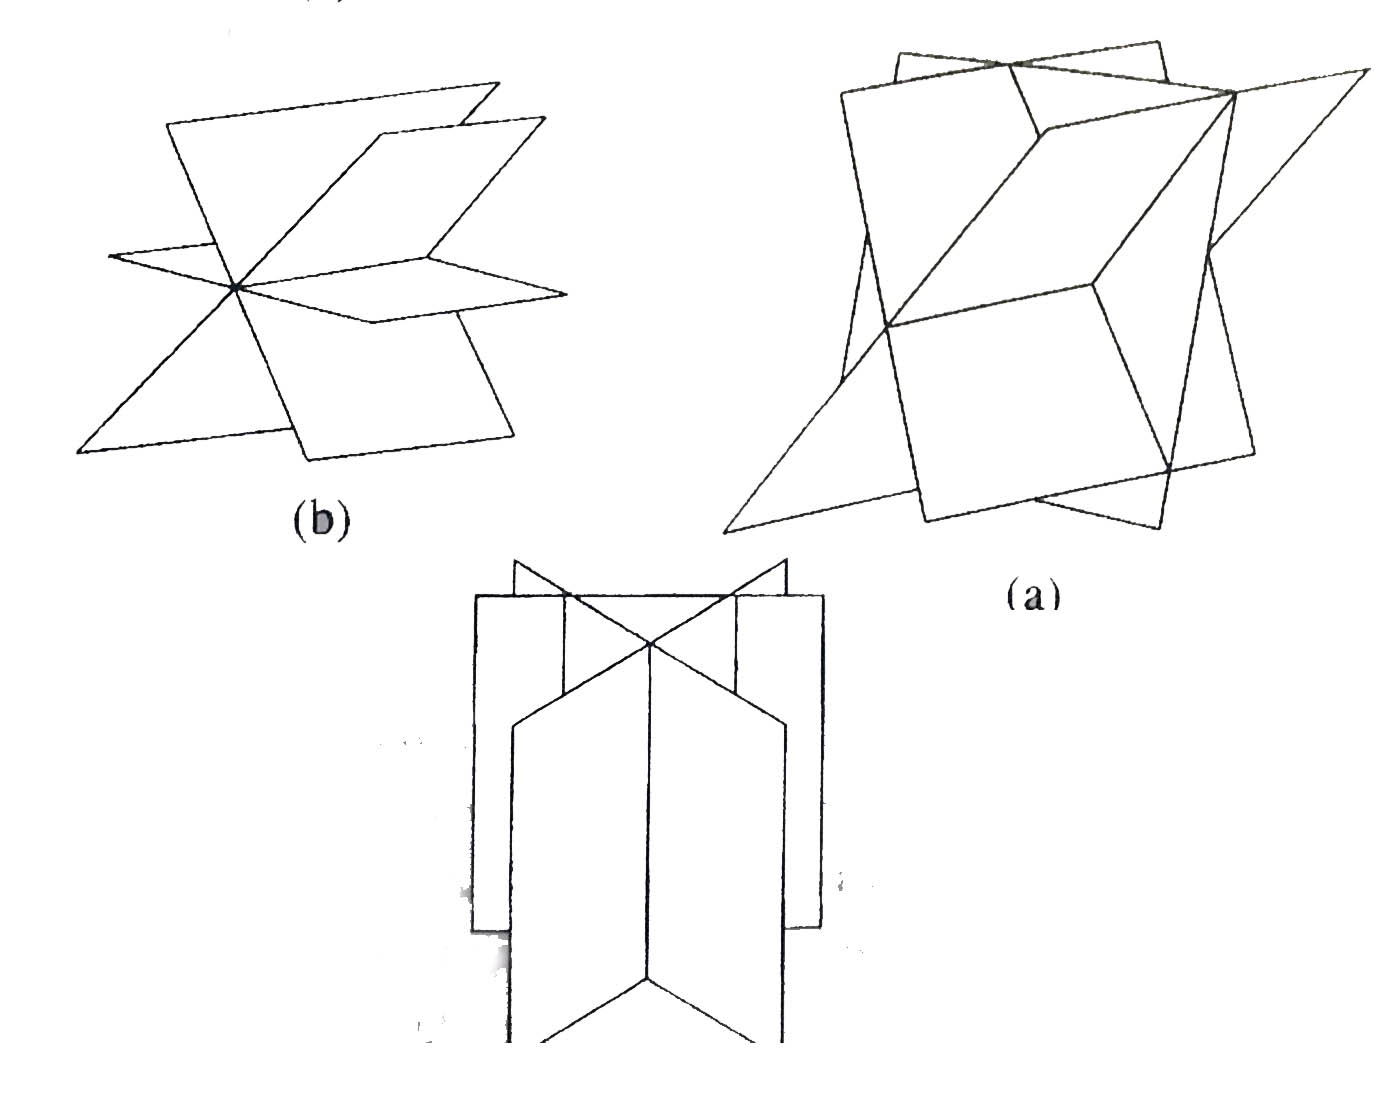
\includegraphics[width=0.5\textwidth]{planarint.jpg}
		\caption{Three cases of planes intersecting.}
		\label{fig:planarint}
	\end{figure}
	
\section{Matrix Algebra}
	\subsection{Linear Maps}
		A \textbf{Linear Map} is a function between two vector spaces that preserves addition and scalar multiplication. If $A$ is an $m\times n$ matrix, $T_A(\vec{x})$ maps $\vec{x}$ from $\mathbb{R}^n$ to $\mathbb{R}^m$.
		
	\subsection{Column and Null Spaces}
		\marginnote{Subspace?}The column and null spaces of a matrix $A$ are \textbf{subspaces} - sets $\in \mathbb{R}^m$ that are closed under vector addition and scalar multiplication. It is possible to find a basis for these subspaces of $A$ with elementary row operations.
		
		\marginnote{Column space?}To find a basis for the \textbf{column space} of $A$, or the subspace of all vectors that can be created through any linear combination of the columns of $A$, first express $A$ in row-reduced echelon form. The columns of the pivot elements in the original $A$ form the basis for the column space, and the pivot columns themselves form the basis for the \textbf{null space}.
		
		\marginnote{Null space?}The null space of $A$ is the solution to $rref(A) = 0$ and is the set of all vectors that when mapped by $A$ yield $\vec{0}$. The number of free variables represents the \textbf{nullity} of $A$, or the size of the vector basis of $ker(A)$, and the \textbf{rank} of $A$ is the number of non-zero rows in $rref(A)$.
		
	\subsection{Transpose Matrices}
		\begin{equation}
			A^T_{ij} = A_{ji}
		\end{equation}
		
		\subsubsection{Fundamental Theorem of Linear Algebra}
			$ker(A)\in\mathbb{R}^n, C(A)\in\mathbb{R}^m, ker(A^T)\in\mathbb{R}^m,C(A^T)\in\mathbb{R}^n$.
			
			\marginnote{Fundamental subspaces?}These are the four fundamental subspaces. All vectors in $C(A)$ are orthogonal to all vectors in $ker(A^T)$ and all vectors in $ker(A)$ are orthogonal to all vectors in $C(A^T)$.
			
			Thus, the solvability of any system $A\vec{x} = \vec{b}$ requires that $\vec{b}\in C(A)$, or, in other words, $\vec{b}\perp ker(A^T)$ (Fredhold Alternative).
	
	\subsection{Matrix Multiplication}
		\marginnote{Matrix multiplication?}If $A$ is $m\times n$ and $b$ is $n\times p$, the matrix product $AB$ is the $m\times p$ matrix $C$ where $c_{ij}$ is the dot product of the $i$\textsuperscript{th} row of $A$ and the $j$\textsuperscript{th} column of $B$. In summation notation, where $k$ runs over the column index of $A$ and the row index of $B$:
		\begin{equation}
			AB_{ij} = \sum_{k=1}^n a_{ik}b_{kj}
		\end{equation}
		
		Note that matrix multiplication is not in general commutative. There are 4 basic properties of matrix multiplication, listed below.
		\begin{center}
			\begin{tabular}{r|l}
				Law							& Example\\\hline
				Right distributive			& $(A+B)C = AC+BC$\\
				Left distributive			& $C(A+B) = CA+CB$\\
				Scalar commutativity		& $(tA)B=t(AB)=A(tB)$\\
				Associative					& $A(BC)=(AB)C$
			\end{tabular}
		\end{center}
		
		\subsection{Identity Matrix}
			An identity matrix is a square matrix with 1s on its \textbf{main diagonal} and 0s elsewhere, and has the following property.
			\begin{equation}
				IA=AI=A
			\end{equation}
			
		\subsection{Matrix Polynomials}
			If $A$ is a square matrix, then we can raise $A$ to powers, where $A^0$ is the identity matrix.
			
\section{Inverse Matrices}
	If $A$ and $B$ are square matrices with equal dimensions and $AB = I$, then $B$ is an \textbf{inverse} of $A$ and $A$ is an \textbf{invertible} matrix.
	\begin{equation}
		AA^{-1} = A^{-1}A = I
	\end{equation}
	If $A$ is invertible, then the system of equations $A\vec{x}=b$ has a unique solution $\vec{x}=A^{-1}b$. In particular, $\vec{x}=\vec{0}$ is the only solution to $A\vec{x}=\vec{0}$.
	
	For a 2-by-2 matrix, it is invertible if its \textbf{determinant} $ad-bc$ is not zero.
	\begin{equation}
		\left(\begin{matrix}
			a&b\\c&d
		\end{matrix}\right)^{-1} = \frac{1}{ad-bc}\left(\begin{matrix}
			d&-b\\-c&a
		\end{matrix}\right)
	\end{equation}
	
	For larger matrices, use basic row operations and \textbf{row rearrangement} to transform the matrix $A$ into the identity matrix $I$, while performing the exact same sequence of steps on $I$ to get $A^{-1}$.
	
	\textbf{Diagonal matrices} and \textbf{upper triangular matrices} are invertible only if there are no zeroes on the main diagonal. In the latter case, it is easier to reduce the columns working from right to left.
	\begin{equation}
		\begin{pmatrix}
			b_1 & 0 & 0\\
			0 & b_2 & 0\\
			0 & 0 & b_3
		\end{pmatrix}
	\end{equation}
	\begin{equation}
		\begin{pmatrix}
			b_11 & b_12 & b_13\\
			0 & b_22 & b_23\\
			0 & 0 & b_33
		\end{pmatrix}
	\end{equation}
	
	\subsection{Projections}
		\marginnote{Project vector to plane?}Given two linearly independent vectors $\vec{a}_1, \vec{a}_2$ and a plane defined by their span, we can find the projection $\vec{p}$ of a vector $\vec{b}$.
		\begin{IEEEeqnarray}{rCl}
			\nonumber\vec{p} & = & c_1\vec{a}_1 + c_2\vec{a}_2\\
			\nonumber\vec{b} - \vec{p} & \perp & \vec{a}_1, \vec{a}_2\\
			\nonumber\vec{a}_1\cdot(\vec{b}-\vec{p}) & = & 0\\
			\nonumber\vec{a}_2\cdot(\vec{b}-\vec{p}) & = & 0\\
			\nonumber A & = & \{\vec{a}_1,\vec{a}_2\}\\
			\vec{p} = A\vec{c} & = & A(A^TA)^{-1}A^T\vec{b}
		\end{IEEEeqnarray}
	
\section{Determinants}
	\marginnote{Determinant equation?}\begin{equation}
		\text{det} A = \sum_{j=1}^n (-1)^{i+j}A_{ij}\cdot \text{det} M_{ij}
	\end{equation}
	\marginnote{Matrix minor?}$M_{ij}$ represents the $ij\textsuperscript{th}$ \textbf{minor} of the $n\times n$ matrix $A$ obtained by removing the $i\textsuperscript{th}$ row and $j\textsuperscript{th}$ column. This is a recursive solution to determinants.
	\begin{lstlisting}[autogobble=true]
		determinant(A):
			if n == 2:
				return A[1,1]*A[2,2] - A[1,2]*A[2,1]
			
			result = 0
			i = 1;	#Can be anything
			for j in A:
				if i+j % 2:
					result -= A[i,j]*determinant(minor(A))
				else:
					result += A[i,j]*determinant(minor(A))
					
			return result
	\end{lstlisting}
	
	\subsection{Properties}
		\begin{itemize}
			\item The formula works for any value $i$ between 1 and $n$.
			\item It is also fine to use $i$ as the controlling variable in the sum.
			\marginnote{Multilinearity?}\item The determinant is \textbf{multilinear} in rows and columns.
			\item If any row or column is multiplied by a scalar $\lambda$, $\text{det} A = \lambda\text{det} A$.
			\marginnote{Alternating?}\item Alternating: switching any two rows or columns flips the sign of the determinant.
			\item $\text{det} A = 0$ if row or columns are linearly dependent.
			\marginnote{$detAB=?$}\item $\text{det} AB = \text{det} A\cdot\text{det} B$
			\marginnote{$detA^{-1}=?$}\item $\text{det} A^{-1} = \dfrac{1}{\text{det} A}$
		\end{itemize}
		Multilinearity: if $A=\{\vec{u_1}, \vec{u_2},\ldots,\vec{u_n}\}$ and $\vec{v}\in\mathbb{R}^n$:
		\begin{equation}
			det\{\vec{u_1}, \vec{u_2},\ldots\vec{u_k}+\vec{v},\ldots,\vec{u_n}\} = det A + det\{\vec{u_1},\ldots,\vec{u_{k-1}},\vec{v},\vec{u_{k+1}},\ldots\vec{u_n}\}
		\end{equation}
		
		Note also that the determinant is equal to the scalar triple product of a $3\times 3$ matrix and the cross product of the column vectors of a $2\times 2$ matrix. In general, the determinant represents the volume of the hypercube bound by the column vectors of $A$.
		
	\subsection{Cramer's Rule}
		\marginnote{Cramer's Rule?}If $det A\neq 0$, and where $\tilde{A}_{ij} = -1^{i+j}\cdot detM_{ij}$
		\begin{equation}
			A^{-1} = \frac{1}{det A}\cdot \tilde{A}^T
		\end{equation}
		
\section*{Important Concepts}
	\subsection*{Matrix Algebra}
		\subsubsection*{Vector Spaces}
			\begin{itemize}
				\item Subspaces are subsets that are closed under certain operations.
				\item The column space is the subspace of all vectors that can be created through linear combinations of column vectors.
				\item The pivot elements of a matrix in rref form correspond to the vector basis of its column space.
				\item The basis for the null space is the column vectors containing pivot elements of rref(A).
				\item Nullity is the number of pivot elements in $rref(A)$ and rank is the number of nonzero rows in $rref(A)$.
			\end{itemize}
			
		\subsubsection*{Matrix Multiplication}
			\begin{itemize}
				\item The number of columns in $A$ must equal the number of rows in $B$.
				\item $C_{ij}$ is given by the dot product of the $i\textsuperscript{th}$ row of $A$ and the $j\textsuperscript{th}$ column of $B$.
			\end{itemize}
			
	\subsection*{Inverse Matrices}
		Cramer's Rule: If $det A\neq 0$, and where $\tilde{A}_{ij} = -1^{i+j}\cdot detM_{ij}$
		\begin{equation}
			A^{-1} = \frac{1}{det A}\cdot \tilde{A}^T
		\end{equation}
		
		A matrix is only invertible if its determinant is nonzero.
		
	\subsection*{Determinants}
		\begin{equation}
			\text{det} A = \sum_{j=1}^n (-1)^{i+j}A_{ij}\cdot \text{det} M_{ij}
		\end{equation}
		
		$M_{ij}$ is the minor made by removing the $i\textsuperscript{th}$ row and $j\textsuperscript{th}$ column of $A$.
		
		\begin{itemize}
			\item Multilinearity
			\item Alternating 
			\item $detAB = detA\cdot detB$
			\item $detA^{-1}=(detA)^{-1}$.
		\end{itemize}
		
%	\begin{center}
%	\begin{tikzpicture}
%		[scale=3,line cap=round,
%		%Styles
%		axes/.style=,
%		important line/.style={very thick},
%		information text/.style={rounded corners,fill=red!10,inner sep=1ex},
%		dot/.style={circle,inner sep=1pt,fill,label={#1},name=#1}			
%		]
%		
%		%Colors
%		\colorlet{anglecolor}{green!50!black}	%angle arcs/lines
%		
%		%The graphic
%	\end{tikzpicture}
%	\end{center}

%	\begin{figure}[htb]
%		\centering
%		\includegraphics[width=0.8\textwidth]{filename.eps}
%		\caption{Caption.}
%		\label{fig:figure}
%	\end{figure}

%		\def\enotesize{\normalsize}
%		\theendnotes
\end{document}